
% This LaTeX was auto-generated from an M-file by MATLAB.
% To make changes, update the M-file and republish this document.

\documentclass{article}
\usepackage{graphicx}
\usepackage{color}
\usepackage{listings}
\usepackage[framed]{mcode}
\usepackage{fullpage}
\usepackage{hyperref}
\usepackage{amsmath}

\definecolor{lightgray}{gray}{0.5}
\setlength{\parindent}{0pt}

\begin{document}

    
    \begin{par}

\title{BE 521 - Homework 6\\{\normalsize Spring 2015}}
\author{Mike Lautman}
\date{\today}
\maketitle
\textbf{Objective:} Spike Sorting

\end{par}
\begin{lstlisting}
clf; close all; clear; clc;
me = 'mlautman';
pass_file = 'mla_ieeglogin.bin';

dataset1 = 'I521_A0006_D001';
[T, session1] = evalc('IEEGSession(dataset1, me, pass_file)');
data1 = session1.data;
durration1 = data1.channels(1).get_tsdetails.getDuration;       % ms
% we must hard code a voltage conversion factor because the ts_details are
% incorrect.
Vconv1 = 1000; %data1.channels(1).get_tsdetails.getVoltageConversion;   % V
sr1 = data1.sampleRate;     % Hz
Nvals1 = data1.channels(1).get_tsdetails.getNumberOfSamples;
nerve = data1.getvalues(1:Nvals1, 2)/Vconv1;
muscl = data1.getvalues(1:Nvals1, 1)/Vconv1;
\end{lstlisting}
\begin{par}

\section*{1 Spike Detection and Clustering}
In this section, you will explore some basic filtering and spike
thresholding to ultimately compare spike clusters you pick out by eye to
those selected by an automated algorithm.

\end{par}
\begin{par}

\subsection*{1.1 Elliptic Filter}

\end{par}
\begin{lstlisting}
order = 4;
% Pass band Ripple in dB
Rp = .1;
% Stop band Ripple in dB
Rs = 40;
% Edge frequency in Hz
e_f = 300;
% Normalized Edge frequency in pi * rad/sample
Wp = e_f * 2 / sr1;
% Design 4th order high pass filter
[b,a] = ellip(order, Rp, Rs, Wp, 'high');

% for output
numerators = b
denominators = a
\end{lstlisting}

\color{lightgray} \begin{lstlisting}
numerators =

    0.3420   -1.2740    1.8676   -1.2740    0.3420


denominators =

    1.0000   -1.7432    1.6167   -0.6559    0.1430

\end{lstlisting} \color{black}
\begin{par}

\subsection*{1.2a Plot Filtered Signals}

\end{par}
\begin{lstlisting}
% Timestamp of last point in the plot in ms
plot_tlen = 50;
% Index of last point in the plot
plot_len = plot_tlen * sr1 / 1000;

% create high pass digital filter

f = filter(b, a, nerve);
ff = filtfilt(b, a, nerve);

% time stamps for plot
ts = (1:plot_len)/sr1;


figure(1)
% Plot raw signal
subplot(2,1,1)
hold on
plot(ts, nerve(1:plot_len))
title('Unfiltered Nerve signal')
xlabel('Time (s)')
ylabel('Voltage (V)')
ylim([-20 50]);

% plot filter and filtfilt signals
subplot(2,1,2)
hold on
title('Filtered Nerve signal')
xlabel('Time (s)')
ylabel('Voltage (mV)')
plot(ts, f(1:plot_len), 'b')
plot(ts, ff(1:plot_len), 'r')
legend('"filter"ed', '"filtfilt"ed')
ylim([-20 50]);
\end{lstlisting}


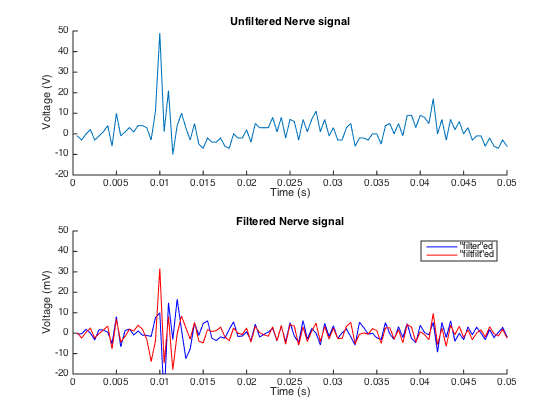
\includegraphics [width=4in]{mlautman_hw6_01.png}
\begin{par}

\subsection*{1.2b Differences in Unfiltered and Filtered Signals}
The unfiltered signal has significant DC offset and a visible 60hz
wave component. The filter'ed and filtfilt'ed signals do not have these
components. The filter'ed signal has significant ringing for the first
15ms and has a small DC component while the filtfilt'ed signal does not
have significant ringing and no significant DC component.

\end{par}
\begin{par}

\subsection*{1.2c Differences in filter and filtfilt Methods}
While the filtfilt function performs a zero-phase digital filtering on
the data in both the forward and reverse directions, the filter function
only performs a rational transfer function in the forward direction.
In teh context of spike detection, ringing can be extremely problematic
because it can cause false positives. For that reason, whenever possible,
one should chunk their signal and use filtfilt for spike detection.

\end{par}
\begin{par}

\subsection*{1.3 Peak Detection}

\end{par}
\begin{lstlisting}
% Find peaks that are over +30 mV
figure(2)
hold on

% plot filtfilt signal
ts = (1:Nvals1)/sr1;
title('Peak Detection on a Filtered Nerve signal')
xlabel('Time (s)')
ylabel('Voltage (mV)')
plot(ts, ff, 'b')
% ylim([-20 50]);

% mark the peaks
[pks , i] = findpeaks(ff .* (ff > 30));
ts = i/sr1;
hold on
title('Filtered Nerve signal')
xlabel('Time (s)')
ylabel('Voltage (mV)')
scatter(ts, pks + 10, 'r.')
xlim([0, 2.500]);
legend('Filtered signal', 'Spike')
\end{lstlisting}


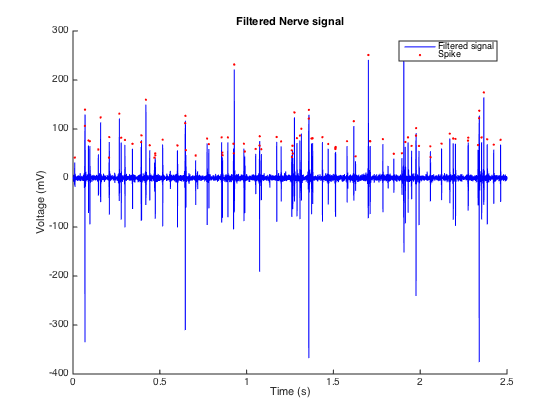
\includegraphics [width=4in]{mlautman_hw6_02.png}
\begin{par}

\subsection*{1.4 Isolating The 3 Nerves}

\end{par}
\begin{lstlisting}
% Cluster the Spikes by Their Amplitude
[pks1 , i1] = findpeaks(ff .* (ff > 30) .* (ff < 85));
ts1 = i1/sr1;
[pks2 , i2] = findpeaks(ff .* (ff >= 85) .* (ff < 200));
ts2 = i2/sr1;
[pks3 , i3] = findpeaks(ff .* (ff >= 200));
ts3 = i3/sr1;


figure(3)
hold on

% plot filtfilt signal
ts = (1:Nvals1)/sr1;
plot(ts, ff, 'b')

% Mark the peaks
scatter(ts1, pks1 + 10, 'r.')
scatter(ts2, pks2 + 10, 'g.')
scatter(ts3, pks3 + 10, 'k.')

% Formatting
title('Handlabeled Source Neurons')
xlabel('Time (s)')
ylabel('Voltage (mV)')
xlim([0, 2.500]);
ylim([-20, 250])
legend(...
    'Filtered signal', 'Neuron 1 Spike', 'Neuron 2 Spike', ...
    'Neuron 3 Spike',  'Location', 'northwest')
\end{lstlisting}


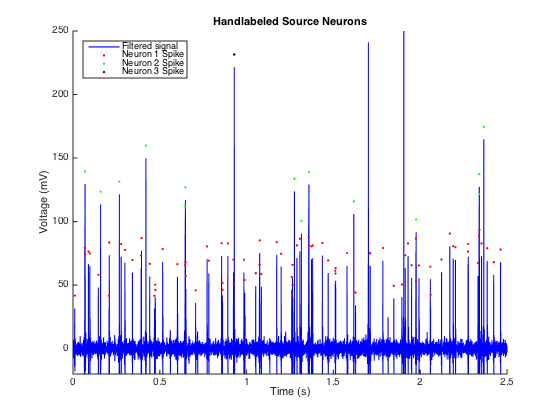
\includegraphics [width=4in]{mlautman_hw6_03.png}
\begin{par}

\subsection*{1.5a K-Means Labeles}

\end{par}
\begin{lstlisting}
% K-means
[idx, c]= kmeans(pks, 3);

% Plot
figure(4)
hold on

% plot filtfilt signal
ts = (1:Nvals1)/sr1;
plot(ts, ff, 'b')


% Plot our handcoded classes
scatter(ts1, pks1 + 10, 'r.')
scatter(ts2, pks2 + 10, 'g.')
scatter(ts3, pks3 + 10, 'k.')

% Plot K-Means classes
[cs, order] = sort(c);
for index=1:3
    ptr = find(order==index);
    mask = find(idx==ptr);
    if index == 1
        scatter(i(mask)/sr1, pks(mask) + 20, 'r*');
    end
    if index == 2
        scatter(i(mask)/sr1, pks(mask) + 20, 'g*');
    end
    if index == 3
        scatter(i(mask)/sr1, pks(mask) + 20, 'k*');
    end
end

% Formatting
title('Source Neurons (HC = hand coded labels, KC = K-means labels)')
xlabel('Time (s)')
ylabel('Voltage (mV)')
xlim([0, 2.500]);
ylim([-20, 300])
legend(...
    'Filtered signal',...
    'Neuron 1 (HC)', 'Neuron 2 (HC)', 'Neuron 3 (HC)',...
    'Neuron 1 (KC)', 'Neuron 2 (KC)', 'Neuron 3 (KC)',...
    'Location', 'northwest')
\end{lstlisting}


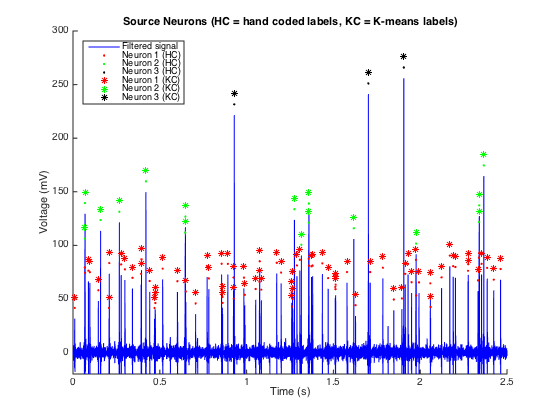
\includegraphics [width=4in]{mlautman_hw6_04.png}
\begin{par}

\subsection*{1.5b Manual vs Clustering}
My hand labeling was nearly exactly the same as the unsupervised
clustering method.

\end{par}
\begin{par}

\subsection*{1.6a Neuron Spike Amplitude and Muscle Potential Change}

\end{par}
\begin{lstlisting}
deltas = zeros(size(i));
for index = 1:length(deltas)
    s = i(index);
    e = min(s + 25, Nvals1);
    deltas(index) = max(muscl(s:e)) - min(muscl(s:e));
end

figure(5)
hold on

% plotting the three types of neuron firings using the K-means clusters
for index=1:3
    ptr = find(order==index);
    mask = find(idx==ptr);
    if index == 1
        scatter(pks(mask), deltas(mask), 'r*');
    end
    if index == 2
        scatter(pks(mask), deltas(mask), 'g*');
    end
    if index == 3
        scatter(pks(mask), deltas(mask), 'k*');
    end
end


% Formatting
title('Neuron Spike Amplitude and Muscle Potential Change')
xlabel('Spike Amplitude (mV)')
ylabel('Muscle Potential Change (mV)')
legend(...
    'Neuron 1 (KC)', 'Neuron 2 (KC)', 'Neuron 3 (KC)',...
    'Location', 'best')
\end{lstlisting}


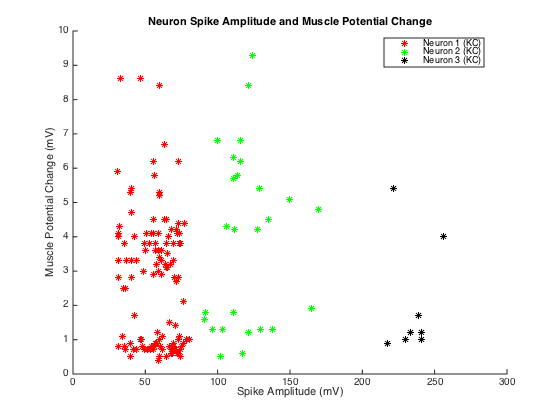
\includegraphics [width=4in]{mlautman_hw6_05.png}
\begin{par}

\subsection*{1.6b}
This plot does not provide convincing evidence that muscle fiber
responses are only due to a subset of the cells. The scatter plot does
not show any strong corrolation between certain cells and muscle
potential changes. Further inspection of the raw muscle response shows
that the noisy signal is very hard to match up against the neuron
firings.

\end{par}
\begin{par}

\section*{2 Multivariate Clustering}

\end{par}
\begin{lstlisting}
dataset2 = 'I521_A0006_D002';
[T, session2] = evalc('IEEGSession(dataset2, me, pass_file)');
data2 = session2.data;
% we must hard code a voltage conversion factor because the ts_details are
% incorrect.
Vconv2 = data2.channels(1).get_tsdetails.getVoltageConversion;   % V
sr2 = data2.sampleRate;     % Hz
Nvals2 = data2.channels(1).get_tsdetails.getNumberOfSamples;
vals = data2.getvalues(1:Nvals2, 1)/Vconv2;
\end{lstlisting}
\begin{par}

\subsection*{2.1a Spikes}

\end{par}
\begin{lstlisting}
% clean for nan vals
vals = vals(~isnan(vals));

% Compute mean and std
Vave = mean(vals(~isnan(vals)));
Vstd = std(vals(~isnan(vals)));


% Store all of the spikes in a single matrix
[Vpks, Vipks] = findpeaks( vals .* ((vals-Vave)/Vstd > 6));
win = round(sr2/1000);
Vspk = zeros(length(Vpks), win * 2 + 1);
for index = 1: length(Vpks)
    Vspk(index,:) = vals(Vipks(index)-win : Vipks(index)+win );
end

ts = -1:1/win:1;

figure(6)
plot(ts, Vspk', 'b')

% Formatting
title('EEG spikes overlayed')
xlabel('Time (ms)')
ylabel('Voltage (mV)')
\end{lstlisting}


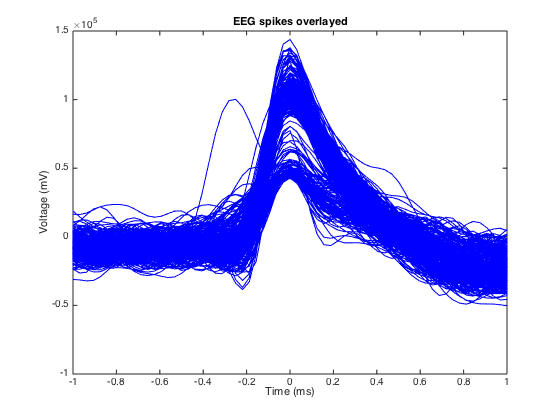
\includegraphics [width=4in]{mlautman_hw6_06.png}
\begin{par}

\subsection*{2.1b}
It seems that there are at least two types of spikes in the data. This
cam be seen by the two heavy blue bands in the middle of the peak. If
there was only one type of spike present, we would expect to see spikes
with variance spread evenly along the verticle axis in the middle of the
plot. Since the variance is clearly bimodal, we can reasonably assert
that there are two types of spikes in the dataset.

\end{par}
\begin{par}

\subsection*{2.2a PCA}

\end{par}
\begin{lstlisting}
% We could get the principal components by using PCA; however, we lose the
% basis in matlabland in doing so.
coeff = pca(Vspk);
% We use SVD to get the orthogonal basis that most efficiently separates
% our data.
[U,S,V] = svd(Vspk);
% We then project our data into this new space
Vpca = Vspk * V;

figure(7)
scatter(Vpca(:,1), Vpca(:,2));

% Formatting
title('EEG spikes in PC space')
xlabel('PC 1')
ylabel('PC 2')
\end{lstlisting}


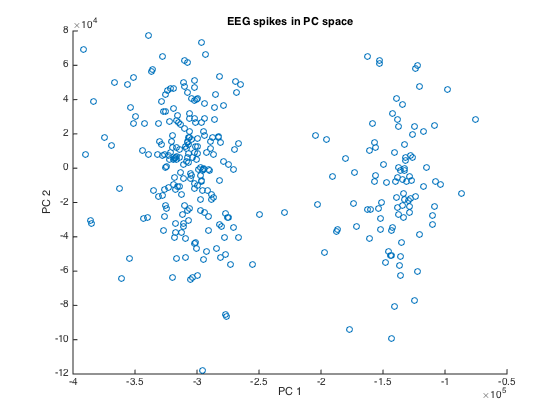
\includegraphics [width=4in]{mlautman_hw6_07.png}
\begin{par}

\subsection*{2.2b Total Variance Explained}

\end{par}
\begin{lstlisting}
% Calculate Variance Explained
VE = sum(S)/sum(sum(S));

% The total variance explained by the top two principal components
TVE_top2 = sum(VE(1:2))

figure(8)
plot(1:length(VE), VE)
title('principal component vs total variance explained')
xlabel('Component')
ylabel('Total Variance Explained')
\end{lstlisting}

\color{lightgray} \begin{lstlisting}
TVE_top2 =

    0.5811

\end{lstlisting} \color{black}


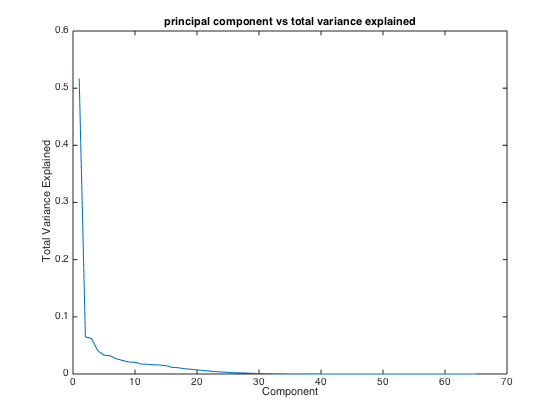
\includegraphics [width=4in]{mlautman_hw6_08.png}
\begin{par}

\subsection*{2.2c}
There are definitely two clusters of spikes

\end{par}
\begin{par}

\subsection*{2.3 K-medians}

\end{par}
\begin{lstlisting}
[idx, C] = kmeans(Vpca(:,1:2), 2, 'Distance', 'cityblock');
mask1 = find(idx==1);
mask2 = find(idx==2);

figure(9)
hold on
scatter(Vpca(mask1,1), Vpca(mask1,2),'r');
scatter(Vpca(mask2,1), Vpca(mask2,2),'g');

% Formatting
title('EEG spikes in PC space')
xlabel('PC 1')
ylabel('PC 2')
\end{lstlisting}


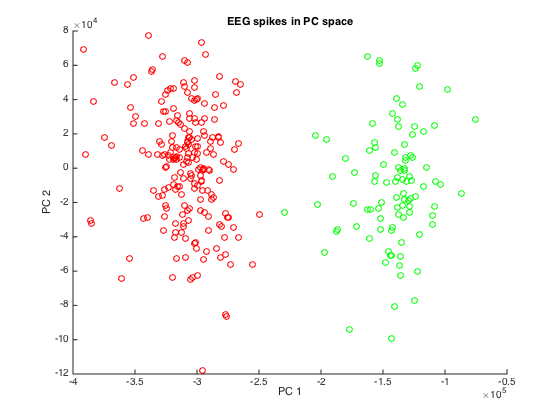
\includegraphics [width=4in]{mlautman_hw6_09.png}
\begin{par}

\subsection*{2.4 K-medians}

\end{par}
\begin{lstlisting}
ts = -1:1/win:1;

figure(6)
hold on
lr = plot(ts, Vspk(mask1,:)', 'r');
lg = plot(ts, Vspk(mask2,:)', 'g');

% Formatting
title('Two types of EEG spikes overlayed')
xlabel('Time (ms)')
ylabel('Voltage (mV)')
legend([lr(1),lg(1)],'Cluster 1','Cluster 2', 'Location', 'northeast')
\end{lstlisting}


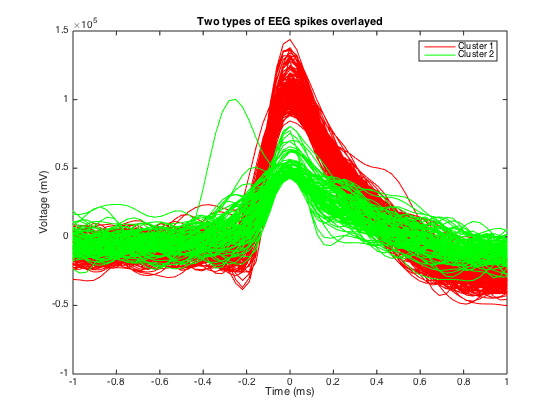
\includegraphics [width=4in]{mlautman_hw6_10.png}

	\subsection*{2.5 DANGER ZONE} One danger of using K-means comes from the fact that K-means is very sensitive to initial conditions. For instance, while running K-medians, I was able to get an incorrect split in the data where the top half of each cluster was red and the bottom half was green. A second issue with K-means is that it does not provide as much information as alternative unsupervised clustering algorithms such as Gaussian Mixture Models. GMM's give the user statistics such as the variance within a cluster along each principle axis as part of the computation. A third danger of using K-means as an unsupervised learning technique is that the programmer must have some prior knowledge about the number of classes in their dataset. This makes K-means unappealing for exploratory data analysis. For these reasons, K-means is really only ever used for tasks when speed of computation is vital or when the technician is content with less than state-of-the-art results.





\end{document}
    
